\section{Mathematical Modelling}

Modelling of the Crazyflie in terms of kinematics and dynamics is done by considering a moving rigid body with 6 degrees-of-freedom (DOF). It results in the equations of motion further used to generate the transfer functions of the system for controlling the Crazyflie. \\

There are different coordinate and reference frames describing the attitude of the drone which are mentioned below along with the transformations between these frames. These transformations are important because different states of the drone are described in reference to other frames.

\subsection{Reference Frames}

A coordinate frame is transformed into another by simple rotations and translations. This is necessary as the 12 states of interest are determined by different frames as it can be seen in the table \ref{table:state_variables}. In this section the following reference frames are explained:

\begin{itemize}
    \item \textbf{Inertial Frame $\mathcal{F}^i$}
    \item Vehicle Frame $\mathcal{F}^v$
    \item Vehicle-1 Frame $\mathcal{F}^{v1}$
    \item Vehicle-2 Frame $\mathcal{F}^{v2}$
    \item \textbf{Body Frame $\mathcal{F}^b$}
\end{itemize}

The rotation matrices are used to get from one frame to another but understanding how these are generated is important for the order of multiplication. 

\begin{table}[H]
 \centering
 \begin{tabular}{|l|l|}
 \hline
    State & Frame \\
 \hline
    $p_x$ & East position in $\mathcal{F}^i$ \\
 \hline
    $p_y$ & North position in $\mathcal{F}^i$ \\
 \hline
    $p_z$ & Up position in $\mathcal{F}^i$  \\
 \hline
    $u$ & Translational velocity along $x^b$ in $\mathcal{F}^b$ \\
 \hline
    $v$ & Translational velocity along $y^b$ in $\mathcal{F}^b$ \\ 
 \hline
    $w$ & Translational velocity along $z^b$ in $\mathcal{F}^b$ \\
 \hline
    $\phi$ & Euler roll angle in $\mathcal{F}^{v2}$ \\
 \hline
    $\theta$ & Euler pitch angle in  $\mathcal{F}^{v1}$ \\
 \hline
    $\psi$ & Euler yaw angle in $\mathcal{F}^v$ \\
 \hline
    $p$ & Roll rate along $x^b$ in $\mathcal{F}^b$ \\ 
 \hline
    $q$ & Pitch rate along $y^b$ in $\mathcal{F}^b$ \\ 
 \hline
    $r$ & Yaw rate along $z^b$ in $\mathcal{F}^b$ \\ 
 \hline
\end{tabular}
 \caption{State variables for a 6DOF rigid body and reference frames.}
  \label{table:state_variables}
\end{table}



\subsubsection{Inertial Frame \texorpdfstring{$\mathcal{F}^{i}$}{Inertial Frame}}

This frame is Earth fixed or fixed to the global system of reference, i.e. lab, and has the unit vector $x^i$ towards the East, $j^i$ towards the North and $k^i$ towards the sky. This represents the East-North-Up (ENU) coordinate frame used for land vehicles as opposed to the aeronautics conventions for North-East-Down (NED) frame. The ENU frame is used as this is described by the drone's firmware.\\

\subsubsection{Vehicle Frame \texorpdfstring{$\mathcal{F}^{v}$}{Vehicle Frame}}

The origin of this frame is at the center of mass (COM) and it coincides with the inertial frame separated only by a translation due to negligible directional differences \cite{beard2012small}. The translation between the two frames can be seen in Figure \ref{figure:frame_inertial}.

\begin{figure}[H]
\centering
 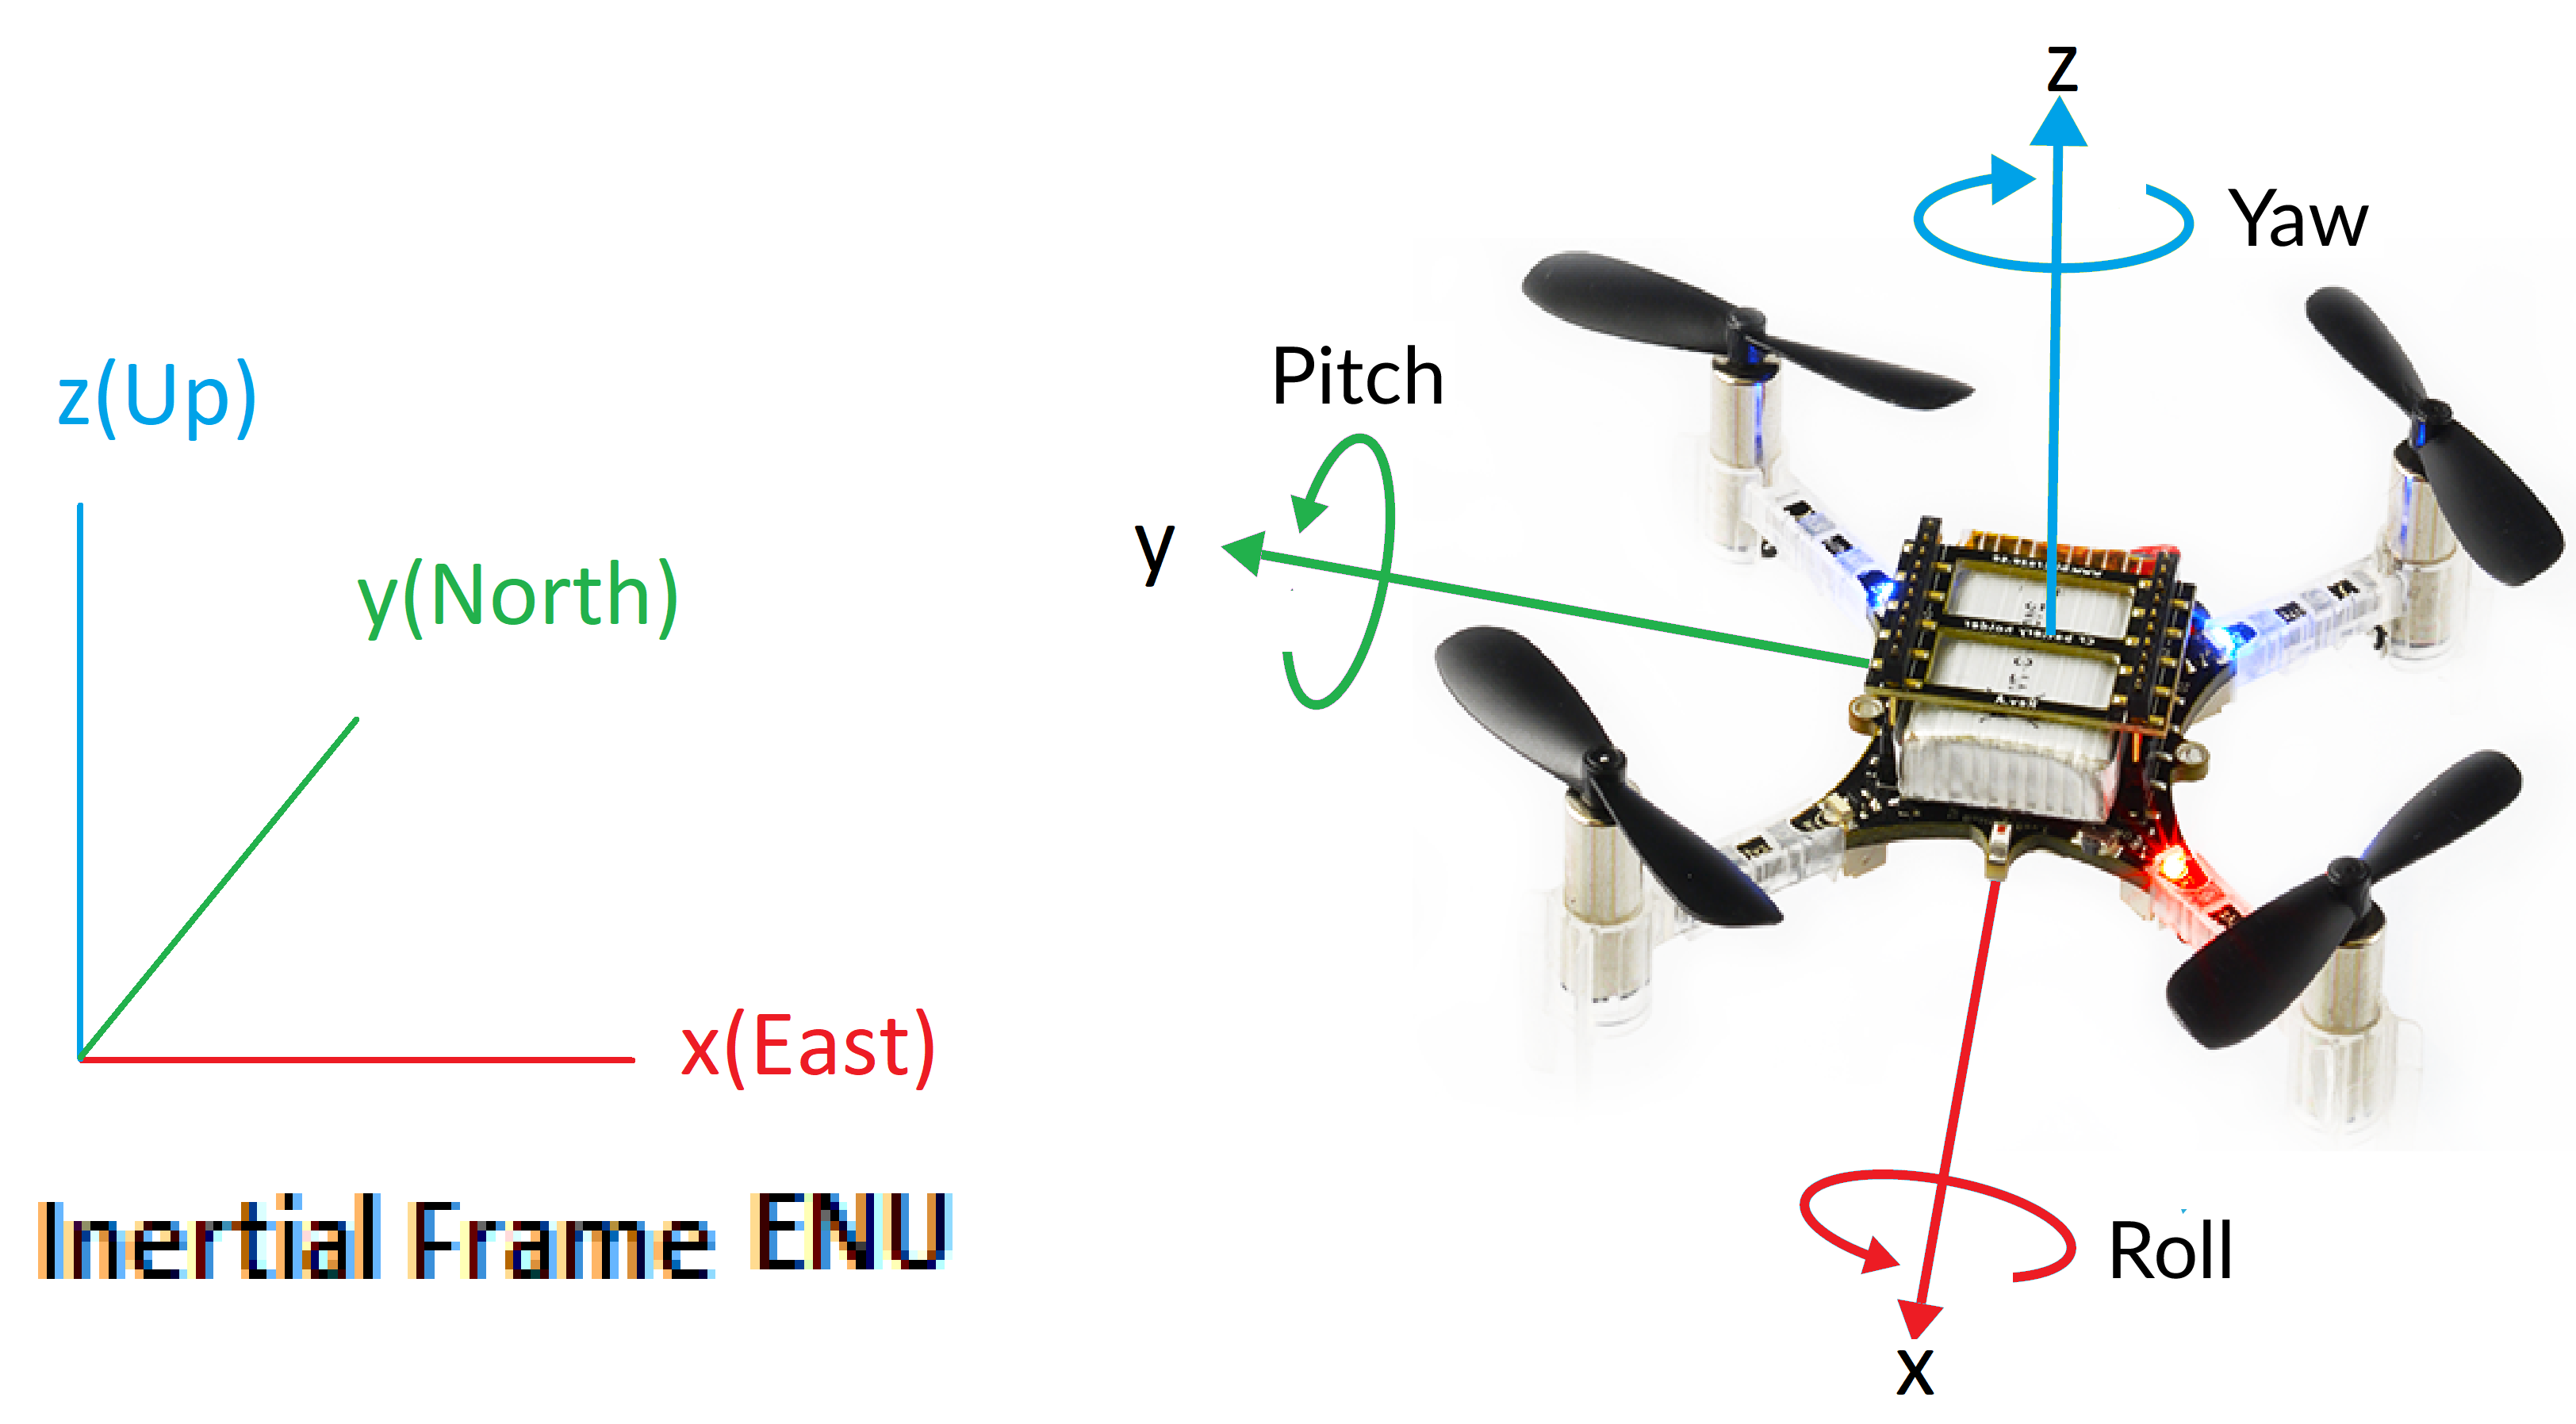
\includegraphics[width=0.7\textwidth]{Figures/frames_crazyflie.png}
 \caption{The inertial frame ENU is laboratory fixed and vehicle frame is drone fixed.}
 \label{figure:frame_inertial}
\end{figure}

\subsubsection{Vehicle-1 Frame \texorpdfstring{$\mathcal{F}^{v1}$}{Vehicle-1 Frame}}
 The vehicle-1 frame has its origin in COM and is described by a positive right-handed rotation about \textbf{z}${^v}$ by the yaw angle $\psi$.
 The rotation matrix ${R}^{v1}_{v}(\psi)$ between $\mathcal{F}^v$ and $\mathcal{F}^{v1}$ is\cite{beard2012small}:
 
\begin{equation*}
    \mathcal{R}^{v1}_{v}(\psi) = \begin{pmatrix}
    \cos\psi & \sin\psi & 0\\
    -\sin\psi & \cos\psi & 0\\
    0 & 0 & 1
    \end{pmatrix}
\end{equation*}

\subsubsection{Vehicle-2 Frame \texorpdfstring{$\mathcal{F}^{v2}$}{Vehicle-2 Frame}}
The vehicle-2 frame continues from vehicle-1 frame and describes a positive rotation about the \textbf{y}$^{v1}$ axis by the pitch angle $\theta$. The rotation matrix ${R}^{v2}_{v1}(\theta)$ from $\mathcal{F}^{v1}$ to $\mathcal{F}^{v2}$ is given by \cite{beard2012small}:

\begin{equation*}
    \mathcal{R}^{v2}_{v1}(\theta) = \begin{pmatrix}
        \cos\theta & 0 & -\sin\theta\\
        0 & 1 & 0\\
        \sin\theta & 0 &\cos\theta\\
    \end{pmatrix}
\end{equation*}
 
\subsubsection{Body Frame \texorpdfstring{$\mathcal{F}^b$}{Body Frame}}

This frame is obtained by rotating $\mathcal{F}^{v2}$ frame about \textbf{i}$^{v2}$ by the roll angle $\phi$. The rotation from $\mathcal{F}^{v2}$ to $\mathcal{F}^{b}$ is given by matrix ${R}^{b}_{v2}(\phi)$ \cite{beard2012small}:

\begin{equation*}
    \mathcal{R}^{b}_{v2}(\phi) = \begin{pmatrix}
        1 & 0 & 0\\
        0 & \cos\phi & \sin\phi &\\
        0 & -\sin\phi & \cos\phi
    \end{pmatrix}
\end{equation*}

The final transformation from the vehicle/inertial frame to the body frame can be found by multiplying all rotation matrices above as such:
\begin{align}
\label{equation:trans_body_to_vehicle}
    \mathcal{R}_{v}^{b}(\phi, \theta, \psi) &= \mathcal{R}_{v2}^b(\phi)\mathcal{R}_{v1}^{v2}(\theta)\mathcal{R}_v^{v1}(\psi) &\\
    &= \begin{pmatrix}
        1 & 0 & 0\\
        0 & \cos\phi & \sin\phi &\\
        0 & -\sin\phi & \cos\phi
    \end{pmatrix}
    \begin{pmatrix}
        \cos\theta & 0 & -\sin\theta\\
        0 & 1 & 0\\
        \sin\theta & 0 &\cos\theta
    \end{pmatrix}
    \begin{pmatrix}
    \cos\psi & \sin\psi & 0\\
    -\sin\psi & \cos\psi & 0\\
    0 & 0 & 1
    \end{pmatrix} \nonumber
    \\
    &= \begin{pmatrix}
     \mbox{c}_{\theta}\mbox{c}_{\psi} & \mbox{c}_{\theta}\mbox{s}_{\psi} & -\mbox{s}_{\theta}\\
     \mbox{s}_{\phi}\mbox{s}_{\theta}\mbox{c}_{\psi} - \mbox{c}_{\phi}\mbox{s}_{\psi} & \mbox{s}_{\phi}\mbox{s}_{\theta}\mbox{s}_{\psi} + \mbox{c}_{\phi}\mbox{c}_{\psi} & \mbox{s}_{\phi}\mbox{c}_{\theta}\\
     \mbox{c}_{\phi}\mbox{s}_{\theta}\mbox{c}_{\psi} + \mbox{s}_{\phi}\mbox{s}_{\psi} & \mbox{c}_{\phi}\mbox{s}_{\theta}\mbox{s}_{\psi} - \mbox{s}_{\phi}\mbox{c}_{\psi} & \mbox{c}_{\phi}\mbox{c}_{\theta}
    \end{pmatrix}
\end{align}

\noindent $c_\theta$ is short for $\cos\theta$ and similarly $s_\theta$ is short for $\sin\theta$. The same applies to the other angles.

\subsection{Kinematic Equations}

Kinematics of a rigid body relate position and velocity. A 6 DOF rigid body has 6 positional states, translational and angular, and 6 velocity states, translational and angular. In total there 12 states characterising the drone as seen in Table \ref{table:state_variables}.

\noindent The translational position vector ($P$) in Equation \ref{eq:position_vector} is expressed in the ENU frame and its origin is located at the launch point of the drone.

\begin{equation} \label{eq:position_vector}
	P = [p_x\ p_y\ p_z]^T
\end{equation}

\noindent The translational velocity vector $V$ and the angular velocity vector $\omega$ in Equation \ref{eq:vel_vector} and \ref{eq:angular_vector} are expressed in the body frame.  


\begin{equation} \label{eq:vel_vector}
	V = [u\ v\ w]^T
\end{equation}

\begin{equation} \label{eq:angular_vector}
	\omega = [p\ q\ r]^T
\end{equation}

\noindent The $V$ vector is equal to the time derivatives of the $P$ vector through a rotation from the inertial to the body frame. By inverting the rotation matrix, the time derivatives of $P$ can be expressed in the body frame. The change of frame is shown in Equation \ref{eq:posDot}.

\begin{equation} \label{eq:posDot}
	\dot{P} = \mathcal{R}_{b}^{i} {V}
\end{equation}

\noindent Element-wise Equation \ref{eq:posDot} describes its elements as \cite{article:letter}:

\begin{eqnarray}
	\dot{p_x} &= &(\cos \theta \cos \psi) u + (-\cos\phi \sin\psi + \sin\phi \sin\theta \cos\psi) v\\
	&& +\> (\sin\phi \sin\psi + \cos\phi \sin\theta \cos\psi)w \\
	\dot{p_y} &= & (\cos\theta \sin\psi)u + (\cos\phi \cos\psi + \sin\phi \sin\theta\sin\psi)v \\
	&& +\> (-\sin\phi \cos\psi + \cos\phi \sin\theta \sin\psi)w  \\
	\dot{p_z} &= & (-\sin\theta)u + (\sin\phi \cos\theta)v + (\cos\phi \cos\theta)w 
\end{eqnarray}

On the same line, the angular velocity vector $\omega$ can be expressed by the time derivatives of the Euler angles (Euler rates) through several matrix rotations as the Euler angles are defined in different frames. The Euler rates vector $\dot{\Phi}$ in Equation \ref{eq:position_vector_ang} can be expressed with regards to $\omega$ if the final rotation matrix is inverted.

\begin{equation} \label{eq:position_vector_ang}
	\dot{\Phi} = [\dot{\phi}\ \dot{\theta}\ \dot{\psi}]^T
\end{equation}

The elements of Equation \ref{eq:position_vector_ang} are \cite{article:letter}:

\begin{eqnarray}
	\dot{\phi} & = & p + (\tan\theta \sin\phi)q + (\tan\theta \cos\phi) r \\
	\dot{\theta} &= & (\cos\phi) q - (\sin\phi) r \\
	\dot{\psi} &= & \frac{\sin\phi}{\cos\theta} q + \frac{\cos\phi}{\cos\theta} r
\end{eqnarray}

\subsection{Dynamics Equations}
Deriving the equations of motion for a rigid body implies the use of Newton's second law for linear and rotational motions: $F = ma$ (translational) and $\tau = I \alpha$ (rotational). \\

\subsubsection{The Translational Model}
It was shown above that the inertial linear velocity can be expressed in the body frame: $ V_i^b = [$u$\ $v$\ $w$]^T = [\dot{p_n}\ \dot{p_e}\ \dot{p_d}]^T$ \cite{article:letter}. Since the linear Newton's laws hold in the inertial frame, using the Coriolis equation, the translation motion can be expressed in the body frame:

\begin{equation}  \label{eq:linearforcebodyframe}
	m\frac{dv_i}{dt} = m(\frac{dv_b}{dt} + \omega_{b/i} \times v) = f
\end{equation}

The $\omega_{b/i}$ in Equation \ref{eq:linearforcebodyframe} is the angular velocity in the body frame with respect to the inertial frame. Hence, in body frame elements of Equation \ref{eq:linearforcebodyframe} are given below forming the vector $ \dot{V_i^b} = [\dot{u}\ \dot{v}\ \dot{w}]^T$.

\begin{eqnarray}{}
	\dot{u} &= & rv -qw + \frac{F_{b,x}}{m} \\
	\dot{v} &= & -ru + pw + \frac{F_{b,y}}{m} \\
	\dot{w} &= & qu -pv + \frac{F_{b,z}}{m} 
\end{eqnarray}

The mass of the drone is given by $m$. The force vector $F_b = [F_{b,x}\ F_{b,y}\ F_{b,z}]^T$ represents all forces applied to the drone on each of the axes. The vector is expressed in the body frame.\\

\subsubsection{The Rotational Model}

Similarly, since the rotational Newton's law holds in the inertial frame, using the Coriolis equation the law can be expressed in the body frame as in Equation \ref{eq:rotationalmomentumbodyframe}:

\begin{equation}  \label{eq:rotationalmomentumbodyframe}
	\frac{dh}{dt_i} = \frac{dh}{dt_b} + \omega_{b/i} \times h = \tau
\end{equation}

In Equation \ref{eq:rotationalmomentumbodyframe}, $h$ stands for angular momentum and $\tau$ for applied torque. $h_b$ is the angular momentum in body coordinates and its formula is $h_b = J \omega_{b/i}$, where $J$ is the constant inertia matrix. The inertia matrix $J$ is defined as \cite{beard2012small}:

\begin{equation} \label{eq:J}
	\bm{J} =
	\begin{bmatrix}
		\int(y^2 + z^2)~dm & -\int xy~dm        & -\int xz~dm        \\
		-\int xy~dm        & \int(x^2 + z^2)~dm & -\int yz~dm        \\
		-\int xz~dm        & -\int yz~dm        & \int(x^2 + y^2)~dm
	\end{bmatrix}
\end{equation}

The diagonal terms of the inertia matrix are called $moments$ $of$ $inertia$ while the off-diagonal terms are called $products$ $of$ $inertia$. To simplify equations it is assumed that the quadrotor is symmetric about all three axes, hence $J_{xy}$=$J_{xz}$=$J_{yz}$=0.\cite{beard_quadrotor} This results in the $J$ matrix to be a symmetric matrix:

\begin{equation}\label{eq:inertiaMat}
	\bm{J} = 
	\begin{bmatrix}
		J_x     & 0   & 0 \\
		0       & J_y & 0       \\
		0 & 0   & J_z
	\end{bmatrix}
\end{equation}

Usually the mass properties of a drone are determined using CAD models or pendulum experiments, however if some simplifying assumptions are made about the drone, the moments of inertia can be calculated. The matrix $J$ can be calculated according to Equation \ref{eq:J} assuming the drone is a spherical centre with mass $M$ and radius $R$ with 4 point masses $mr$ located at a distance $l$ from the centre \cite{beard_quadrotor}. The configuration can be seen in Figure \ref{figure:sphericalcenter}.

\begin{figure}[H]
\centering
 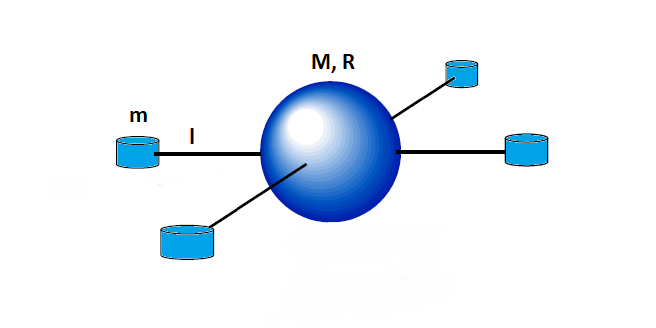
\includegraphics[scale=0.5]{Figures/spherical.png}
 \caption{Drone's moments of inertia assumed as those of a spherical centre. Source: \cite{beard_quadrotor}}
 \label{figure:sphericalcenter}
\end{figure}

The inertia for a solid sphere is given by Equation \ref{eq:inertiamoments} and hence the moments of inertia are given below.

\begin{equation}  \label{eq:inertiamoments}
	J = \frac{2MR^2}{5}
\end{equation}

\begin{eqnarray}{}
	J_x &= & \frac{2MR^2}{5} + 2l^2mr \\
	J_y &= & \frac{2MR^2}{5} + 2l^2mr\\
	J_z &= & \frac{2MR^2}{5} + 4l^2mr 
\end{eqnarray}

The components of the angular accelerations vector $\dot{\omega}$ = $[\dot{p}\ \dot{q}\ \dot{r}]^T$ are  if the torque vector is $\tau = [\tau_\phi\ \tau_\theta\ \tau_\psi]^T$ \cite{beard_quadrotor}:

\begin{eqnarray}{}
	\dot{p} &= & \frac{J_y-J_z}{Jx}qr + \frac{1}{J_x}\tau_\phi\\
	\dot{q} &= & \frac{J_z-Jx}{Jy}pr + \frac{1}{J_y}\tau_\theta \\
	\dot{r} &= & \frac{J_x-J_y}{Jz}pq + \frac{1}{J_z}\tau_\psi 
\end{eqnarray}

The equations derived in this section represent kinematics and dynamics of a 6 DOF rigid body. These equations need to be completed with the forces and moments from a free body diagram.

\subsection{Forces and Moments}

A free-body diagram of the forces and moments acting on a drone can be seen in Figure \ref{figure:freebodydiagram}.

\begin{figure}[H]
\centering
 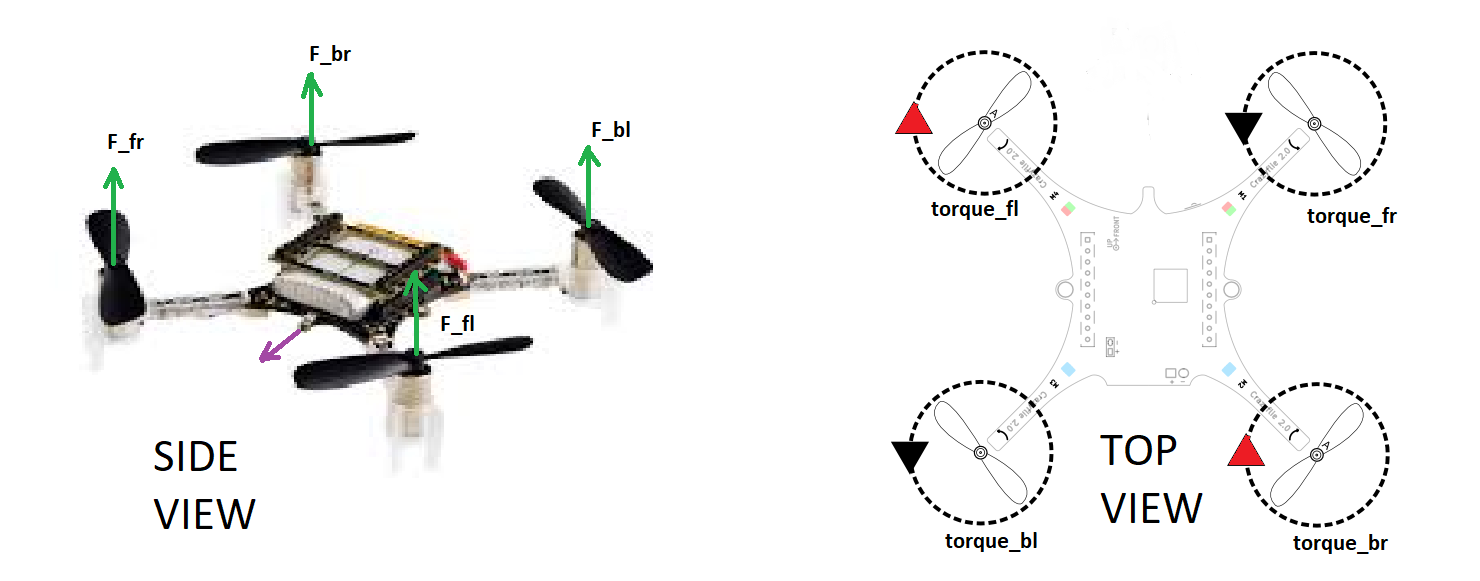
\includegraphics[scale=0.45]{Figures/f_m.png}
 \caption{The free-body diagram of the Crazyflie stating the external forces acting on the drone in the first picture from the left. There is also a gravitational force acting on the z-axis of the drone. In the second picture the torques due to the propeller's drag are shown. The rotational direction of the motors has to be pair opposite.}
 \label{figure:freebodydiagram}
\end{figure}

From Figure \ref{figure:freebodydiagram} can be seen that the configuration used coincides with the Crazyflie's design of an "X" configuration meaning the drone flies with two motors in front instead of one as in the "+" configuration.\\

As shown in Figure \ref{figure:freebodydiagram} each motor produces a force and torque. The total thrust force acting on the drone is: $F = F_{fl} + F_{fr} + F_{br} + F_{bl}$, where each component represents the upwards thrust force generated by each propeller. The thrust force is expressed depending on the angular speed ($\delta$) of a propeller as in Equation \ref{eq:angularspeed}:

\begin{equation}  \label{eq:angularspeed}
	T_i = C_T\delta_i^2
\end{equation}

The $C_T$ is a constant thrust coefficient which has to be determined through experiments and $\delta_i$ is the rotational speed of a propeller in revolutions per minute. Given that the direction of the thrust force for all motors is the same, the equation for the total thrust force can be re-written as Equation \ref{eq:thrustforce}:

\begin{equation}  \label{eq:thrustforce}
	F = C_T(\delta_{fl}^2 + \delta_{fr}^2 + \delta_{bl}^2 + \delta_{br}^2)
\end{equation}

\subsubsection{The Translational Model}

The translational model consists of translational acceleration equations on each axis found by using Newton's $2^{nd}$ law. The total force acting on the quadcopter are the thrust forces and the gravitational force $F_g$. The gravitational pull varies with altitude but it is assumed constant at $g$ = 9.805416 $\frac{m}{s^2}$. As the gravity acceleration is always pointing towards Earth's center, opposite to the ENU frame, $F_g$ is written as:

\begin{equation} \label{eq:gravForce}
	\bm{F}_{g} =
	\begin{bmatrix}
		0\\ 0 \\-mg
	\end{bmatrix}
\end{equation}

Expressed in the inertial frame $F_g$ is rotated with the rotation matrix in Equation \ref{equation:trans_body_to_vehicle} to express it in the body frame.

\begin{eqnarray}
	{F}^b_{gx} &= & \sin \theta ~m g \\
	{F}^b_{gy} &= & -\sin \phi \cos \theta ~m g \\
	{F}^b_{gz} &= & -\cos \phi \cos \theta ~m g 
\end{eqnarray}

The gravitational force acts only on the z-axis. As mentioned earlier, Newton's law holds in the inertial frame and all forces must be expressed in body frame. This is simply done by multiplying with the rotation matrix in Equation \ref{equation:trans_body_to_vehicle}. The resulting equations of the translational model are:

\begin{eqnarray}{}
	m\ \ddot{px} &= & -F^b\sin\theta\\
	m\ \ddot{py} &= & F^b\cos\theta\sin\phi \\
	m\ \ddot{pz} &= & (F^b+F^b_gz)\cos\phi\cos\theta 
\end{eqnarray}

Further replacing the force vector with Equation \ref{eq:thrustforce} the complete equations for the translational model become:

\begin{eqnarray}{}
	m\ \ddot{p_x} &= & -C_T(\delta_{fl}^2 + \delta_{fr}^2 + \delta_{bl}^2 + \delta_{br}^2)\sin\theta\\
	m\ \ddot{p_y} &= & C_T(\delta_{fl}^2 + \delta_{fr}^2 + \delta_{bl}^2 + \delta_{br}^2)\cos\theta\sin\phi \\
	m\ \ddot{p_z} &= & (C_T(\delta_{fl}^2 + \delta_{fr}^2 + \delta_{bl}^2 + \delta_{br}^2)+F^b_{gz})\cos\phi\cos\theta 
\end{eqnarray}

\subsubsection{The Rotational Model}

To find the equations of motion for the rotational model Newton's second law for rotational motion is used. Each propeller produces a torque and according to Newton's law the sum of the net torque is the product between the moment of inertia and the angular acceleration.\\

Torque is defined as force times distance and when rolling the drone rotates around the x-axis meaning it depends on the thrust forces of motor pairs: to roll to the right, motors front and back on the right have to spin slower than the other pair; to pitch nose down, motors back left and right have to spin faster than the opposite pair; to yaw left cross motor pairs have to alternate motor speeds as motor front-right and motor back-left have to spin faster than the other pair. These motions are described by the following equations:

\begin{eqnarray}{}
    \tau_\phi &= & l \ (-F_{br} - F_{fr} + F_{bl} + F_{fl})\\
	\tau_\theta &= & l\ (F_{br} - F_{fr} + F_{bl} - F_{fl}) \\
	\tau_\psi &= & -\tau_{br} + \tau_{fr} + \tau_{bl} - \tau_{fl}
\end{eqnarray}

%\begin{eqnarray}{}
%	J_x\ddot{\phi} &= & l \ (-F_{br} - F_{fr} + F_{bl} + F_{fl})\\
%	J_y\ddot{\theta} &= & l\ (F_{br} - F_{fr} + F_{bl} - F_{fl}) \\
%	J_z\ddot{\psi} &= & -\tau_{br} + \tau_{fr} + \tau_{bl} - \tau_{fl}
%\end{eqnarray}

%Taking just the coefficient of the force components, the motor mixing matrix (MM) is obtained where $c$ stands for collective meaning all motors spin at the same speed:

%\begin{equation}\label{eq:mixingMat}
%	\bm{MM} = 
%	\begin{bmatrix}
%		c & -\phi & \theta & -\psi \\
%		c & - \phi & -\theta & \psi \\
%		c & \phi &  \theta  & \psi \\
%		c & \phi &  -\theta  & -\psi
%	\end{bmatrix}
%\end{equation}
%In Equation \ref{eq:mixingMat} each row corresponds to a motor starting from top to bottom, the order of the motors is: back-right, front-right, back-left, front-left. This matrix gives the equation to how each motor should move when receiving motor commands. 
As seen earlier that there is a thrust coefficient, the same applies for the drag torque having a drag coefficient $C_D$. The torque is assumed to be proportional to the square of the motor's rotational speed and the rotational equations can be completed:

\begin{eqnarray}{}
	\tau_\phi &= & l \ C_T(-\delta_{br}^2 - \delta_{fr}^2 + \delta_{bl}^2 + \delta_{fl}^2)\\
	\tau_\theta &= & l \ C_T(\delta_{br}^2 - \delta_{fr}^2 + \delta_{bl}^2 - \delta_{fl}^2) \\
	\tau_\psi &= & C_D(-\delta_{br}^2 + \delta_{fr}^2 + \delta_{bl}^2 - \delta_{fl}^2)
\end{eqnarray}

\subsection{Linearization of Motion Models}

Due to the non-linearity of the equations of motion found earlier for both the linear and rotational model, these have to be linearized using the Taylor first order approximation. Linearization is required in order to derive linear controllers for the drone.\\

Using the Equation \ref{eq:taylor} at a linearization point which should be an equilibrium point $\bar{x}$ for the drone, all 6 equations of motion are linearized at the equilibrium point.  

\begin{equation}  \label{eq:taylor}
f(x)\approx f(\bar{x})+{f}'(\bar{x})(x-\bar{x})\rightarrow \Delta f(x) \approx {f}'(\bar{x})\Delta x
\end{equation}

The equations that need to be linearized are partially differentiated in respect to each of the variables as in Equation \ref{eq:taylorexpansion}. As the equations are linearized, they express variations from the linearization point. The symbol $\Delta$ is used in the linearized equations to indicate this.\\

\begin{equation}  \label{eq:taylorexpansion}
\Delta f = \frac{\partial f}{\partial x_1}\mid_{(\bar{x_1}, \bar{x_2}, ...)} \Delta x_1 + \frac{\partial f}{\partial x_2}\mid_{(\bar{x_1}, \bar{x_2}, ...)} \Delta x_2 + ...
\end{equation}

An equilibrium point for a drone is the hovering position where all accelerations and velocities are 0. When inspecting the equations for the linear model it is clear that in order for the accelerations $\ddot{p_x}$ and $\ddot{p_y}$ to be 0 the roll and pitch angles $\phi$ and $\theta$ need to be 0. However, acceleration on the z-axis needs to counteract the gravitational pull in order to hover and having the roll and pitch angles null, from the z-axis equation a constant is determined that specifies the required motors speed in order to maintain hover - see Equation \ref{eq:motorconstant}.

\begin{equation}  \label{eq:motorconstant}
\bar{\delta_i} = \sqrt{\frac{mg}{4C_T}} 
\end{equation}

Simplifying further the equations of motion, assuming small $\phi$ and $\theta$ angles, Euler rates become as in Equation \ref{eq:lin_euler_rates}:

\begin{equation} \label{eq:lin_euler_rates}
	[\dot{\phi}\ \dot{\theta}\ \dot{\psi}]^T = [p\ q\ r]^T
\end{equation}

Assuming that the Coriolis terms $qr$, $pr$, $pq$ are small the angular acceleration vector $\dot{\omega}$ becomes \cite{beard_quadrotor}:

\begin{eqnarray}{}
	\dot{p} &= & \frac{1}{J_x}\tau_\phi\\
	\dot{q} &= & \frac{1}{J_y}\tau_\theta \\
	\dot{r} &= & \frac{1}{J_z}\tau_\psi 
\end{eqnarray}

Having the simplified Euler rates and angular accelerations, the Euler accelerations $[\ddot{\phi}\ \ddot{\theta}\ \ddot{\psi}]^T$ can be found by substituting the Euler rate in the angular acceleration vector.\\

The linearized equations of motion for the translational model are:

\begin{eqnarray}{}
	m\ \Delta \ddot{p_x} &= & -C_T(\bar{\delta_{fl}}^2 + \bar{\delta_{fr}}^2 + \bar{\delta_{bl}}^2 + \bar{\delta_{br}}^2)\Delta\theta\\
	m\ \Delta \ddot{p_y} &= & C_T(\bar{\delta_{fl}}^2 + \bar{\delta_{fr}}^2 + \bar{\delta_{bl}}^2 + \bar{\delta_{br}}^2)\Delta\phi \\
	m\ \Delta \ddot{p_z} &= & C_T(\bar{\delta_{fl}}\Delta\delta_{fl} + \bar{\delta_{fr}}\Delta\delta_{fr} + \bar{\delta_{bl}}\Delta\delta_{bl} + \bar{\delta_{br}}\Delta\delta_{br}) 
\end{eqnarray}


The linearized equations of motion for the rotational model are:

\begin{eqnarray}{}
	J_x\Delta\ddot{\phi} &= & l \ C_T(-\bar{\delta_{br}}\Delta\delta_{br} - \bar{\delta_{fr}}\Delta\delta_{fr} + \bar{\delta_{bl}}\Delta\delta_{bl} + \bar{\delta_{fl}}\Delta\delta_{fl})\\
	J_y\Delta\ddot{\theta} &= & l \ C_T(\bar{\delta_{br}}\Delta\delta_{br} - \bar{\delta_{fr}}\Delta\delta_{fr} + \bar{\delta_{bl}}\Delta\delta_{bl} - \bar{\delta_{fl}}\Delta\delta_{fl}) \\
	J_z\Delta\ddot{\psi} &= & C_D(-\bar{\delta_{br}}\Delta\delta_{br} + \bar{\delta_{fr}}\Delta\delta_{fr} + \bar{\delta_{bl}}\Delta\delta_{bl} - \bar{\delta_{fl}}\Delta\delta_{fl})
\end{eqnarray}

Writing the linearized equation compactly, these become:

\begin{eqnarray}{}
	\ddot{p_x} &= & -g\theta\\
	\ddot{p_y} &= & g\phi \\
	\ddot{p_z} &= & \frac{\Delta F_g}{m}\\
	\ddot{\phi} &= & \frac{l}{J_x}\\
	\ddot{\theta} &= & \frac{l}{J_y} \\
	\ddot{\psi} &= & \frac{1}{J_z}
\end{eqnarray}


In Table \ref{table:parameters} the specifications of the Crazyflie are shown:

% Please add the following required packages to your document preamble:
% \usepackage[table,xcdraw]{xcolor}
% If you use beamer only pass "xcolor=table" option, i.e. \documentclass[xcolor=table]{beamer}
\begin{table}[H]
\begin{tabular}{|l|l|l|}
\hline
\rowcolor[HTML]{C0C0C0} 
\textbf{Parameter} & \textbf{Description}             & \textbf{Value}                               \\ \hline
M                  & Mass of Crazyflie without motor  & 0.2 [Kg]                                 \\ \hline
mr                 & Mass of rotor                    & 0.07 [Kg]                                \\ \hline
m                  & Total mass with Optitrack marker & 0.29 [Kg]                                \\ \hline
l                  & Arm length                       & 0.03973 {[}m{]}                              \\ \hline
R                  & Rotor radius                     & 0.0231348 {[}m{]}                            \\ \hline
J_x                 & Moment of inertia on x-axis      & 2.638\times 10^{-4} [Kg\times m^2] \\ \hline
J_y                 & Moment of inertia on y-axis      & 2.638\times 10^{-4} [Kg\times m^2] \\ \hline
J_z                 & Moment of inertia on z-axis      & 3.585\times 10^{-4} [Kg\times m^2] \\ \hline
C_T               & Thrust coefficient               & 0.2025 \cite{modellingcrazy}                                       \\ \hline
C_D               & Drag coefficient                 & 0.11 \cite{modellingcrazy}                                        \\ \hline
\end{tabular}
\caption{Table of Crazyflie specific parameters.}
\label{table:parameters}
\end{table}

Simulating the linearized equation of motion for the roll angle the resulting angle is shown in Figure \ref{figure:sim_roll}.

\begin{figure}[H]
\centering
 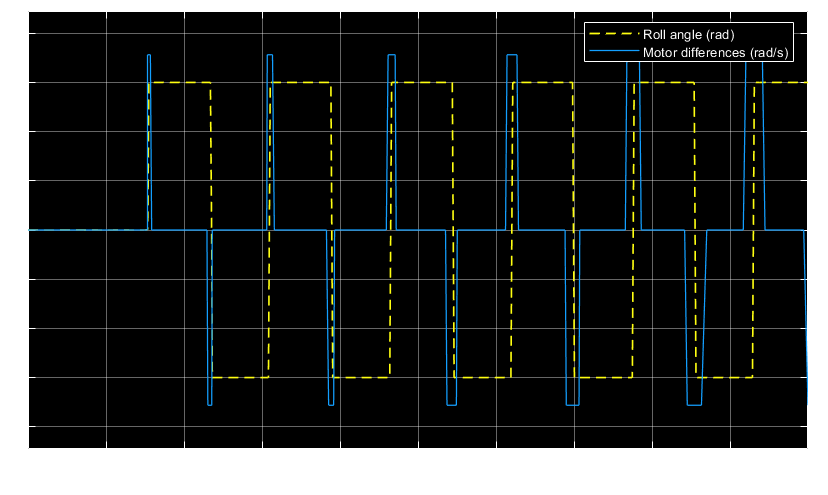
\includegraphics[width=\textwidth]{Figures/lin_roll.png}
 \caption{The simulated roll dynamics of the linearized equation. The roll angle is plotted with the motor pair difference to show the angle change at the change in motors command.}
 \label{figure:sim_roll}
\end{figure}

\section{Control Design}
\label{section:Control}

Having modelled the Crazyflie's dynamics, a translational and rotational controller can be designed in order to control the drone. As controlling the drone is done through a network, a control perspective of the system is shown in Figure \ref{figure:controller_network}.

\begin{figure}[H]
\centering
 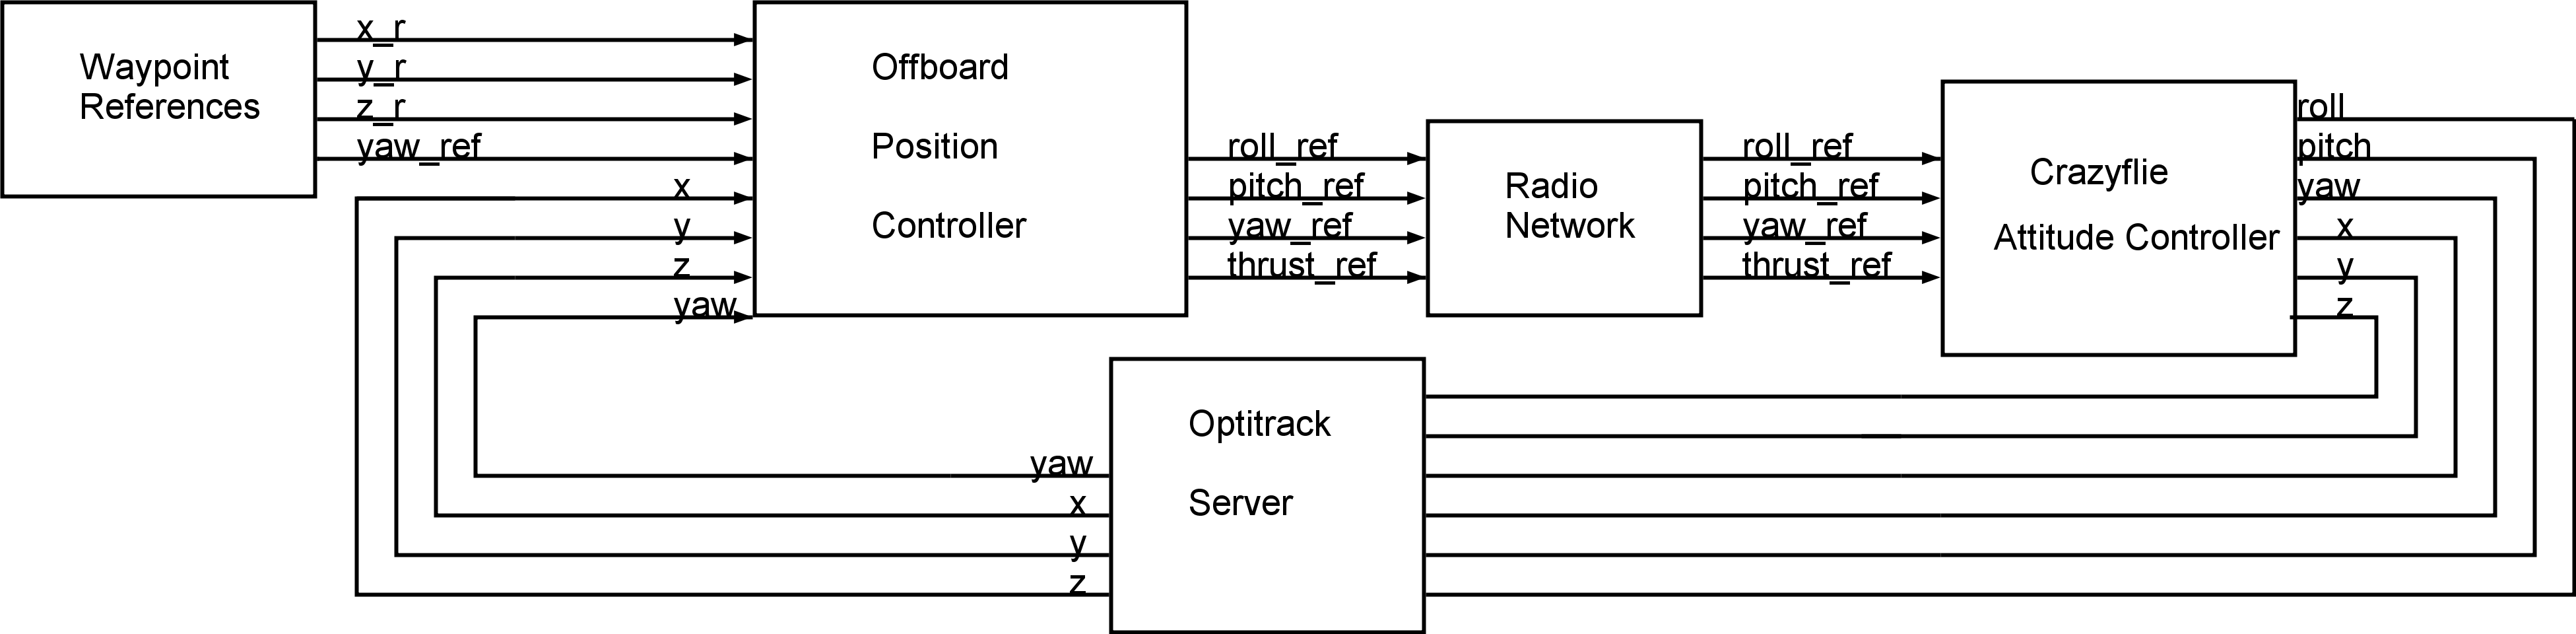
\includegraphics[width=\textwidth]{Figures/updated_network_view.png}
 \caption{A network control perspective over the real-time system.}
 \label{figure:controller_network}
\end{figure}

In this project the two controllers, the trajectory and position (translational) controller are designed offboard while the Crazyflie's internal controller is an attitude controller. This gives the opportunity to analyse the network's influence on the controller when there is network delay and packet loss.\\

For simulation purposes, the network is assumed perfect when designing and tuning the position controller and in later section the network is considered using the Truetime toolbox.\\

Before designing the outer controller, the internal controller of the drone has to be understood so that the right inputs are given to the drone. Figure \ref{figure:internal_controller} shows the inner loop which is the rate controller running at 500 Hz. The outer loop is the attitude controller running at half the speed, 250 Hz. The accepted inputs are the motor commands in PWM. As can be seen from Figure \ref{figure:controller_network} the offboard controller sends as output motor commands.

\begin{figure}[H]
\centering
 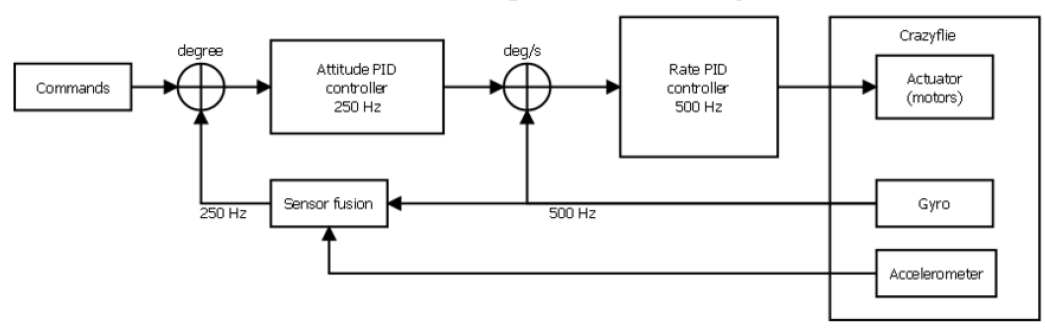
\includegraphics[width=\textwidth]{Figures/internal_controller.png}
 \caption{The internal cascaded attitude controller of the Crazyflie. Inputs to the controller are motor commands in PWM. Source:\cite{modellingcrazy}}
 \label{figure:internal_controller}
\end{figure}

As the internal controller is needed for the simulation, it has been designed in Simulink as an attitude controller shown in Figure \ref{figure:attitude_controller}. Both the attitude and position controller are designed using the classic control theory.

\begin{figure}[H]
\centering
 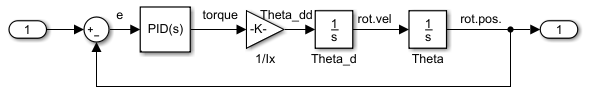
\includegraphics[width=\textwidth]{Figures/attitude_controller.png}
 \caption{The simulated internal roll controller of Crazyflie.}
 \label{figure:attitude_controller}
\end{figure}

In order to control a swarm a drones, trajectory waypoints need to be sent to each of the drone and such waypoints are composed of the coordinates (x, y, z, yaw). The position controller takes as reference input the waypoint coordinates and outputs motor commands for the drones to execute. In the simulation however the position controller outputs the angular displacement which is ultimately passed to the attitude controller. In Simulink the position controller for the x-axis is shown in Figure \ref{figure:position_controller}.

\begin{figure}[H]
\centering
 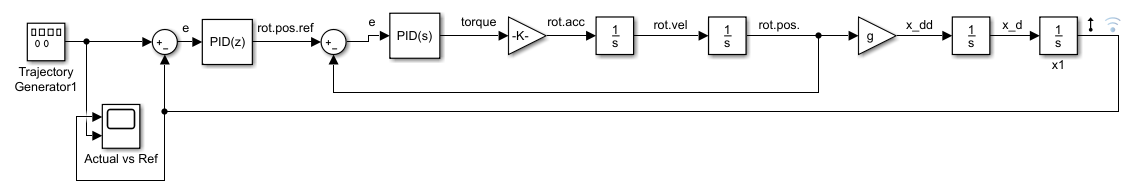
\includegraphics[width=\textwidth]{Figures/pos_contr_simulink.png}
 \caption{The simulated position controller of the x-axis.}
 \label{figure:position_controller}
\end{figure}

The step response of the position controller can be seen in Figure \ref{figure:x_axis}. The controller is stable and converges to steady-state confirmed by the Bode plot of the system in Figure \ref{figure:bode}.

\begin{figure}[H]
\centering
 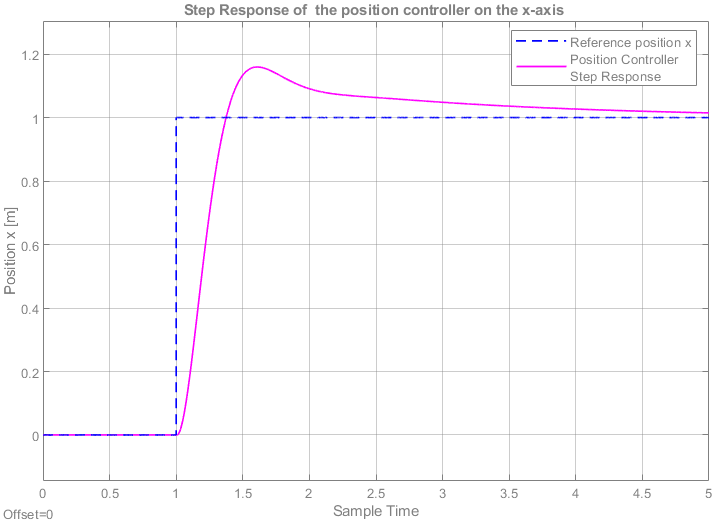
\includegraphics[width=\textwidth]{Figures/x_axis.png}
 \caption{The x-axis position controller step response.}
 \label{figure:x_axis}
\end{figure}

\begin{figure}[H]
\centering
 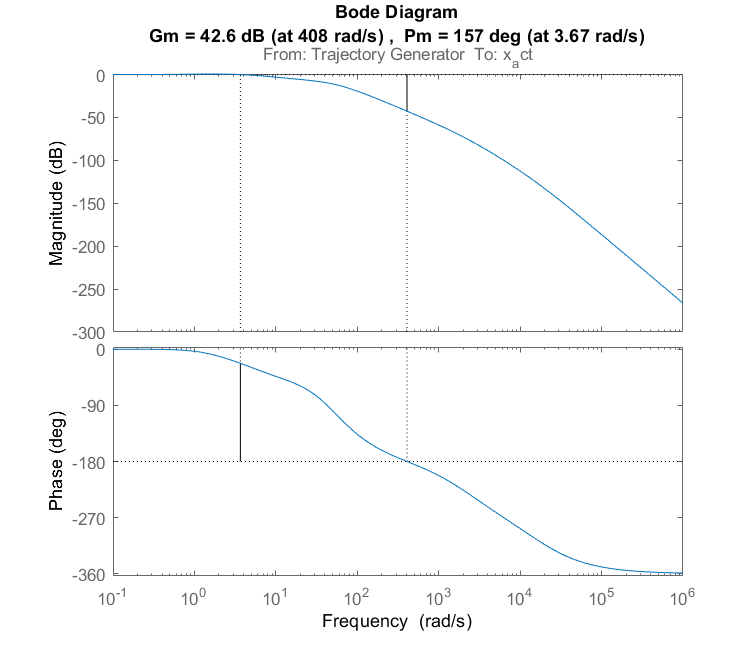
\includegraphics[width=\textwidth]{Figures/bode.png}
 \caption{The Bode plots of the system for the position controller on the x-axis.}
 \label{figure:bode}
\end{figure}

The Bode plot gain and phase margin show that the system is stable. From the crossover frequency the bandwidth of the controller to reach steady-state is given, 407.8865 rad/s or 65 Hz which is close to the frequency of the offboard positional controller sampling at 50 Hz. From the step response, the system reaches steady-state in 3.5 seconds which for a hovering drone is a slow response. The overshoot is 15\% of the steady-state value. \\

In the simulation it was assumed that Crazyflie's internal controller is continuous while the position controller is considered discrete because is implemented on software and is running on another platform than the drone. It has proven difficult to discretize the position controller part of a network loop for which the system would remain stable. This is a well-known issue of discretizing continuous controllers and there are 3 common ways to perform it: forward Euler, backwards Euler and trapezoidal. However, the discrete position discrete controller is given by Equation \ref{eq:discrete}.

\begin{eqnarray}{}
	P &= & K_P * e\\
	I &= & K_I * (I_{prior} + e*z) \\
	D &= & K_D * \frac{e - e_{prior}}{z}
	\label{eq:discrete}
\end{eqnarray}

The output of this controller is y = P + I + D where $e$ stands for current error, $e_{prior}$ stands for last error, $z$ is the sampling time and $K_P$, $K_I$, $K_D$ are the controller's gains.

%The integral term responds to the error build-up mostly due to disturbances unaccounted for such as wind, payload, etc. This term is used to reduce further the steady-state error.